\begin{frame}
  \frametitle{Уравнение Навье-Стокса}

  \begin{block}{Суть уравнения}
    Уравнение Навье-Стокса~--- <<$\vect F=m\vect a$>> для жидкостей.
  \end{block}

  \begin{block}{Для маленького объёма ($V\to 0$)}
    \begin{itemize}
      \item Масса $m=\rho V$, где $\rho$~--- плотность;
      \item Ускорение $\vect a=\frac{d\vect u}{dt}$, где $\vect u$~--- скорость.
    \end{itemize}
  \end{block}

  \begin{block}{Объёмные силы}
    $\vect F=\rho\frac{d\vect u}{dt}$~--- сила, действующая на каждый элементарный объём.
  \end{block}
\end{frame}

\begin{frame}
  \frametitle{Уравнение Навье-Стокса}

  \begin{block}{Силы, входящие в уравнение}
    \begin{itemize}
      \item Силы, возникающие из-за разности давлений;
      \item Силы, возникающие из-за вязкости;
      \item Силы гравитации;
      \item Силы поверхностного натяжения;
      \item Любые другие внешние силы.
    \end{itemize}
  \end{block}
\end{frame}

\begin{frame}
  \frametitle{Давление}

  \begin{block}{Замечание}
    Мы рассматриваем слабосжимаемые жидкости.
    \begin{center}
      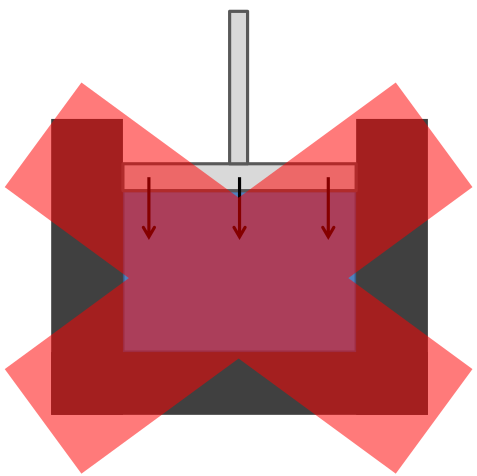
\includegraphics[height=.5\paperheight]{pressure.png}
    \end{center}
  \end{block}
\end{frame}

\begin{frame}
  \frametitle{Давление}

  \begin{block}{Роль давления}
    Силы давления оказывают сопротивление сжатию и расширению.
    \begin{center}
      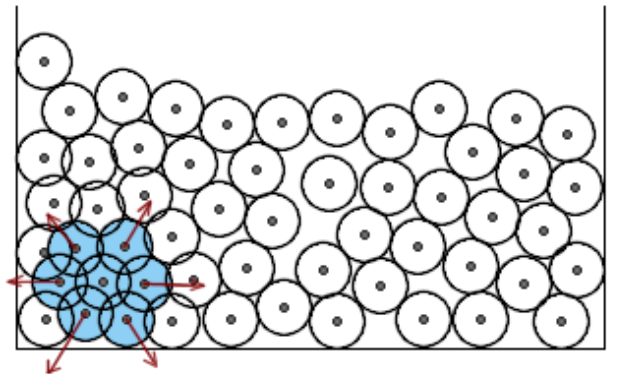
\includegraphics[height=.25\paperheight]{repulse-forces.png}
      \hspace{1.5cm}
      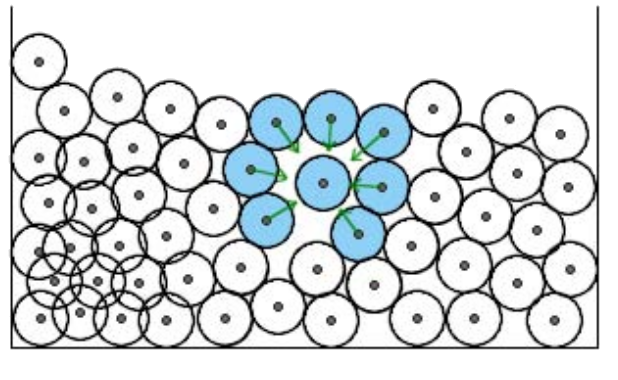
\includegraphics[height=.25\paperheight]{attractive-forces.png}
    \end{center}
  \end{block}

  \begin{block}{Уравнение}
    Разность давлений ведёт к изменению скорости, поэтому
    \[ \vect f^p=-\nabla p. \]
  \end{block}
\end{frame}

\begin{frame}
  \frametitle{Вязкость}

  \begin{block}{Роль вязкости}
    Вязкость ведёт к изменению энергии в результате внутреннего трения. Молекулы диффундируют между слоями жидкости, тем самым уравнивая скорость.
    \begin{center}
      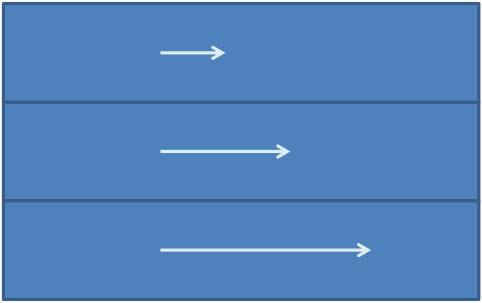
\includegraphics[height=.2\paperheight]{viscosity.png}
    \end{center}
  \end{block}

  \begin{block}{Уравнение}
    Аналитически силы вязкости задаются как
    \[ \vect f^v=\mu\laplace\vect u, \]
    где $\mu$~--- коэффициент вязкости
  \end{block}
\end{frame}

\begin{frame}
  \frametitle{Поверхностное натяжение}

  \begin{block}{Роль поверхностного натяжения}
    Молекулы жидкости находятся под влиянием сил притяжения от соседних молекул, которые уравновешены внутри жидкости.
    \begin{center}
      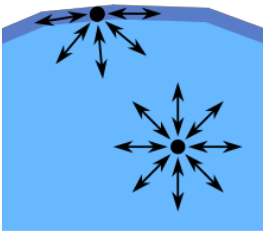
\includegraphics[height=.3\paperheight]{imbalance.png}
    \end{center}
    Однако такая связь ведёт к дисбалансу сил возле поверхности.
  \end{block}
\end{frame}

\begin{frame}
  \frametitle{Поверхностное натяжение}

  \begin{block}{Уравнение}
    Часто силы поверхностного натяжения аппроксимируют как
    \[ \vect f^s=-\sigma k\vect n, \]
    \begin{conditions}
      $\sigma$ & коэффициент поверхностного натяжения;\\
      $k$ & кривизна поверхности;\\
      $\vect n$ & нормаль к поверхности.
    \end{conditions}
  \end{block}

  \begin{block}{Влияние кривизны}
    \centering
    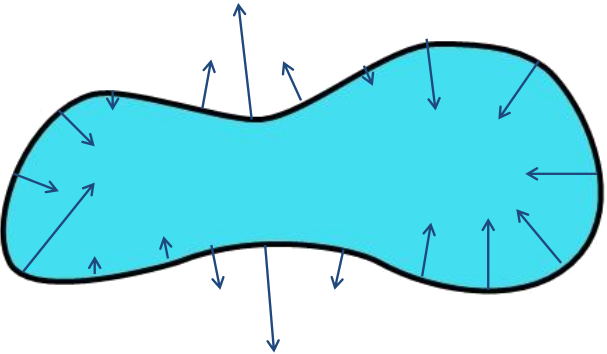
\includegraphics[height=.25\paperheight]{curvature.png}
  \end{block}
\end{frame}

\begin{frame}
  \frametitle{Уравнение Навье-Стокса}

  \begin{block}{Уравнение движения}
    \[ \rho\frac{d\vect u}{dt}=-\nabla p+\mu\laplace\vect u-\sigma k\vect n+\rho\vect g+\vect f_\text{др}, \]
    \begin{conditions}
      $\rho$ & плотность;\\
      $\vect u$ & скорость;\\
      $\mu$ & коэффициент вязкости;\\
      $\sigma$ & коэффициент поверхностного натяжения;\\
      $k$ & кривизна поверхности;\\
      $\vect n$ & нормаль к поверхности;\\
      $\vect g$ & ускорение свободного падения;\\
      $\vect f_\text{др}$ & прочие внешние силы.
    \end{conditions}
  \end{block}

  \begin{block}{Уравнение неразрывности (для несжимаемой жидкости)}
    \[ \nabla\cdot\vect u=0. \]
  \end{block}
\end{frame}

\begin{frame}
  \frametitle{Гидродинамика сглаженных частиц (ГСЧ)}

  \begin{block}{Идея}
    Аппроксимировать решение уравнения Навье-Стокса набором движущихся частиц.

    \begin{center}
      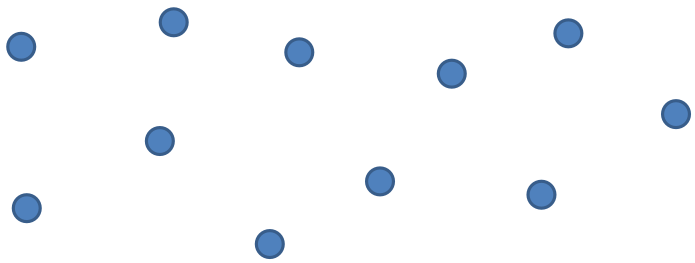
\includegraphics[height=.3\paperheight]{particles.png}
    \end{center}

    Каждая частица имеет массу, скорость и позицию.
  \end{block}
\end{frame}

\begin{frame}
  \frametitle{ГСЧ}

  \begin{block}{Проблема}
    Для аппроксимации непрерывных полей необходимо иметь информацию в любой точке, а не только в выбранных частицах.
  \end{block}

  \begin{block}{Решение}
    <<Разгладим>> информацию частиц в некотором радиусе.

    \begin{center}
      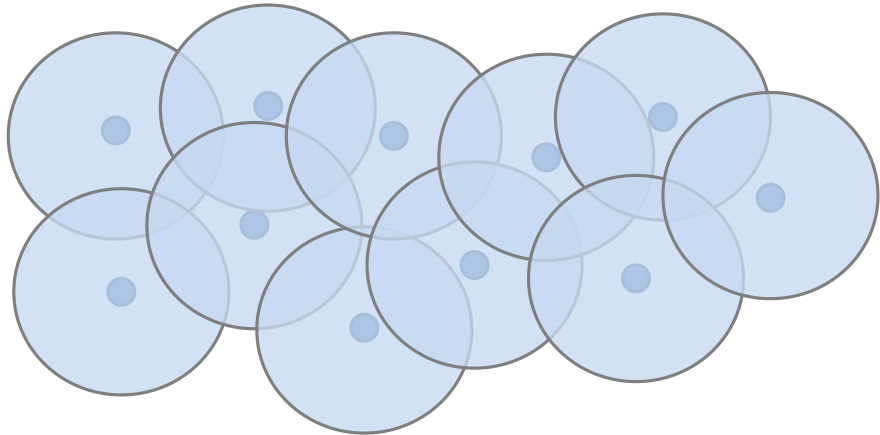
\includegraphics[height=.2\paperheight]{smooth.png}
    \end{center}

    Значение в любой точке может быть получено как взвешенная сумма значений ближайших частиц.
  \end{block}
\end{frame}

\begin{frame}
  \frametitle{Ядра сглаживания}

  \begin{center}
    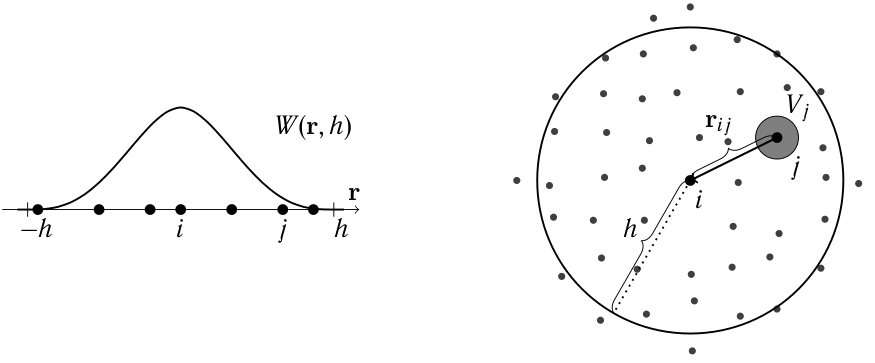
\includegraphics[height=.3\paperheight]{particle-approx.png}
  \end{center}

  \begin{block}{Значение поля}
    \[ f(\vect r_i)\approx\sum_{j=1}^N\frac{m_j}{\rho_j}f(\vect r_j)\kernel(\vect r_i-\vect r_j, h), \]
    \begin{conditions}
      $\kernel$ & ядро сглаживания;\\
      $h$ & радиус сглаживания;\\
      $N$ & кол-во соседних частиц.
    \end{conditions}
  \end{block}
\end{frame}

\begin{frame}
  \frametitle{Ядра сглаживания}

  \begin{block}{Производные поля}
    Аналогичным образом выводится градиент поля:
    \[ \nabla f(\vect r_i)\approx\sum_{j=1}^N\frac{m_j}{\rho_j}f(\vect r_j)\nabla\kernel(\vect r_i-\vect r_j, h). \]

    И лапласиан поля:
    \[ \laplace f(\vect r_i)\approx\sum_{j=1}^N\frac{m_j}{\rho_j}f(\vect r_j)\laplace\kernel(\vect r_i-\vect r_j, h). \]
  \end{block}
\end{frame}

\begin{frame}
  \frametitle{Дискретизация силы давления}

  \begin{block}{Первая попытка}
    \[ \vect f_i^p=-\nabla p(\vect r_i)=-\rho_i\sum_{j\neq i}m_j\frac{p_j}{\rho_j}\nabla\kernel(\vect r_i-\vect r_j, h). \]
  \end{block}

  \begin{block}{Проблема}
    Сила не симметрична (действие $\neq$ противодействию).
  \end{block}

  \begin{block}{Решение}
    Один из способов симметризовать силу:
    \[ \vect f_i^p=-\nabla p(\vect r_i)=-\rho_i\sum_{j\neq i}\left(\frac{p_i}{\rho_i^2}+\frac{p_j}{\rho_j^2}\right)m_j\nabla\kernel(\vect r_i-\vect r_j, h). \]
  \end{block}
\end{frame}

\begin{frame}
  \frametitle{Дискретизация сил давления}

  \begin{block}{Проблема}
    Как определить давление?
  \end{block}

  \begin{block}{Решение}
    \begin{enumerate}
      \item Позволим небольшие колебания плотности;
      \item Определим плотности всех частиц;
      \item Используя уравнение состояния, найдём давление.
    \end{enumerate}
  \end{block}

  \begin{block}{Уравнения состояния}
    \begin{itemize}
      \item Закон идеального газа: $p=k(\rho-\rho_0)$;
      \item Уравнение Тэта: $p=B\big((\frac{\rho}{\rho_0})^7-1\big)$,
    \end{itemize}
    где $k$ и $B$~--- константы.
  \end{block}
\end{frame}

\begin{frame}
  \frametitle{Дискретизация сил вязкости и гравитация}

  \begin{block}{Дискретизация сил вязкости}
    Поскольку силы вязкости зависят только от разности скоростей, а не от их абсолютных значений, то простейший способ симметризовать аппроксимацию~--- использовать разность скоростей:
    \[ \vect f_i^v=\mu\laplace\vect u(\vect r_i)=\mu\sum_{j}(\vect u_j-\vect u_i)\frac{m_j}{\rho_j}\laplace\kernel(\vect r_i-\vect r_j, h). \]
  \end{block}

  \begin{block}{Гравитация}
    Т.к. гравитация не зависит от характеристик частиц, то уравнение гравитационных сил ($\vect f^g=\rho\vect g$) не требует дискретизации.
  \end{block}
\end{frame}

\begin{frame}
  \frametitle{Дискретизация сил поверхностного натяжения}

  \begin{center}
    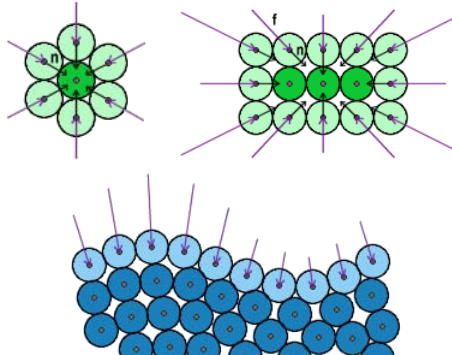
\includegraphics[height=.4\paperheight]{tension.png}
  \end{center}

  \begin{block}{Проблема}
    Необходимо определить кривизну $k$. Какие частицы составляют поверхность?
  \end{block}
\end{frame}

\begin{frame}
  \frametitle{Дискретизация сил поверхностного натяжения}

  \begin{block}{}
    \begin{columns}[onlytextwidth]
      \begin{column}{.7\textwidth}
        Модель для расчёта строится на <<цветовой>> функции:
        \[
          c(\vect r) =
          \begin{cases}
            1, & \exists i: \vect r = \vect r_i\\
            0 & \text{иначе}
          \end{cases}
        \]
      \end{column}
      \begin{column}{.3\textwidth}
        \centering
        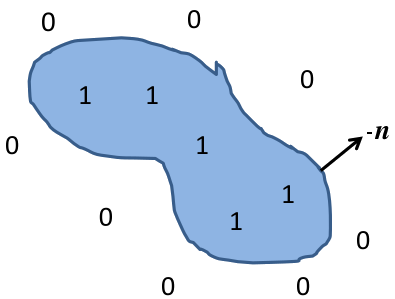
\includegraphics[width=\textwidth]{color.png}
      \end{column}
    \end{columns}

    При этом, внутренняя нормаль вычисляется как
    \[ \vect n_i=\nabla c(\vect r_i)=\sum_j\frac{m_j}{\rho_j}\nabla\kernel_d(\vect r_i-\vect r_j, h). \]

    Тогда сила поверхностного натяжения принимает вид
    \[ \vect f_i^s=-\sigma\laplace c_i\frac{\vect n_i}{|\vect n_i|}. \]
  \end{block}
\end{frame}
